\section{Architecture} \label{architecture}
As mentioned in Section \ref{introduction}, we decided to implement an Android application for mobile phones. Since the Chrome browser offers an interface for using \gls{ble} on the web, we developed a Chrome extension, using the dedicated Web Bluetooth \gls{api} \cite{WebBTAPI}. \\
Through the extension, we inject a button on the website. The button is used to establish a \gls{ble} connection between application and extension. Upon successful pairing, the extension is allowed to read characteristics that are advertised from the app. The characteristics contain username and password, which the extension inserts directly into the login forms of the website.

\noindent Before starting with the implementation we defined minimal requirements of the Android application and the Chrome extension: \\

\noindent Minimal requirements of application:
\begin{itemize}
\item Secure storage of credentials
\item Adding, changing and deleting credentials
\item En- and decryption of data 
\item Authentication through biometric identification
\item Establishing a Bluetooth connection with the web extension
\end{itemize}
\vspace{0.3cm}
\noindent Minimal requirements of extension:
\begin{itemize}
\item Injection of a button onto the website
\item Establishment of \gls{ble} Connection
\item Reading the advertised characteristics
\item Filling credentials into the proper forms
\end{itemize}

The initial workflow between the mobile device and web browser is shown in Figure \ref{fig:comm}. First, the user selects the credential to send to the web browser and authenticates via fingerprint. After this process, the application starts advertising. Upon button click in the web browser, the extension and application start the pairing process. Finally, the credentials are inserted into the forms. \\


\vspace{0.3cm}
\begin{figure}[!htb]
    \centering
    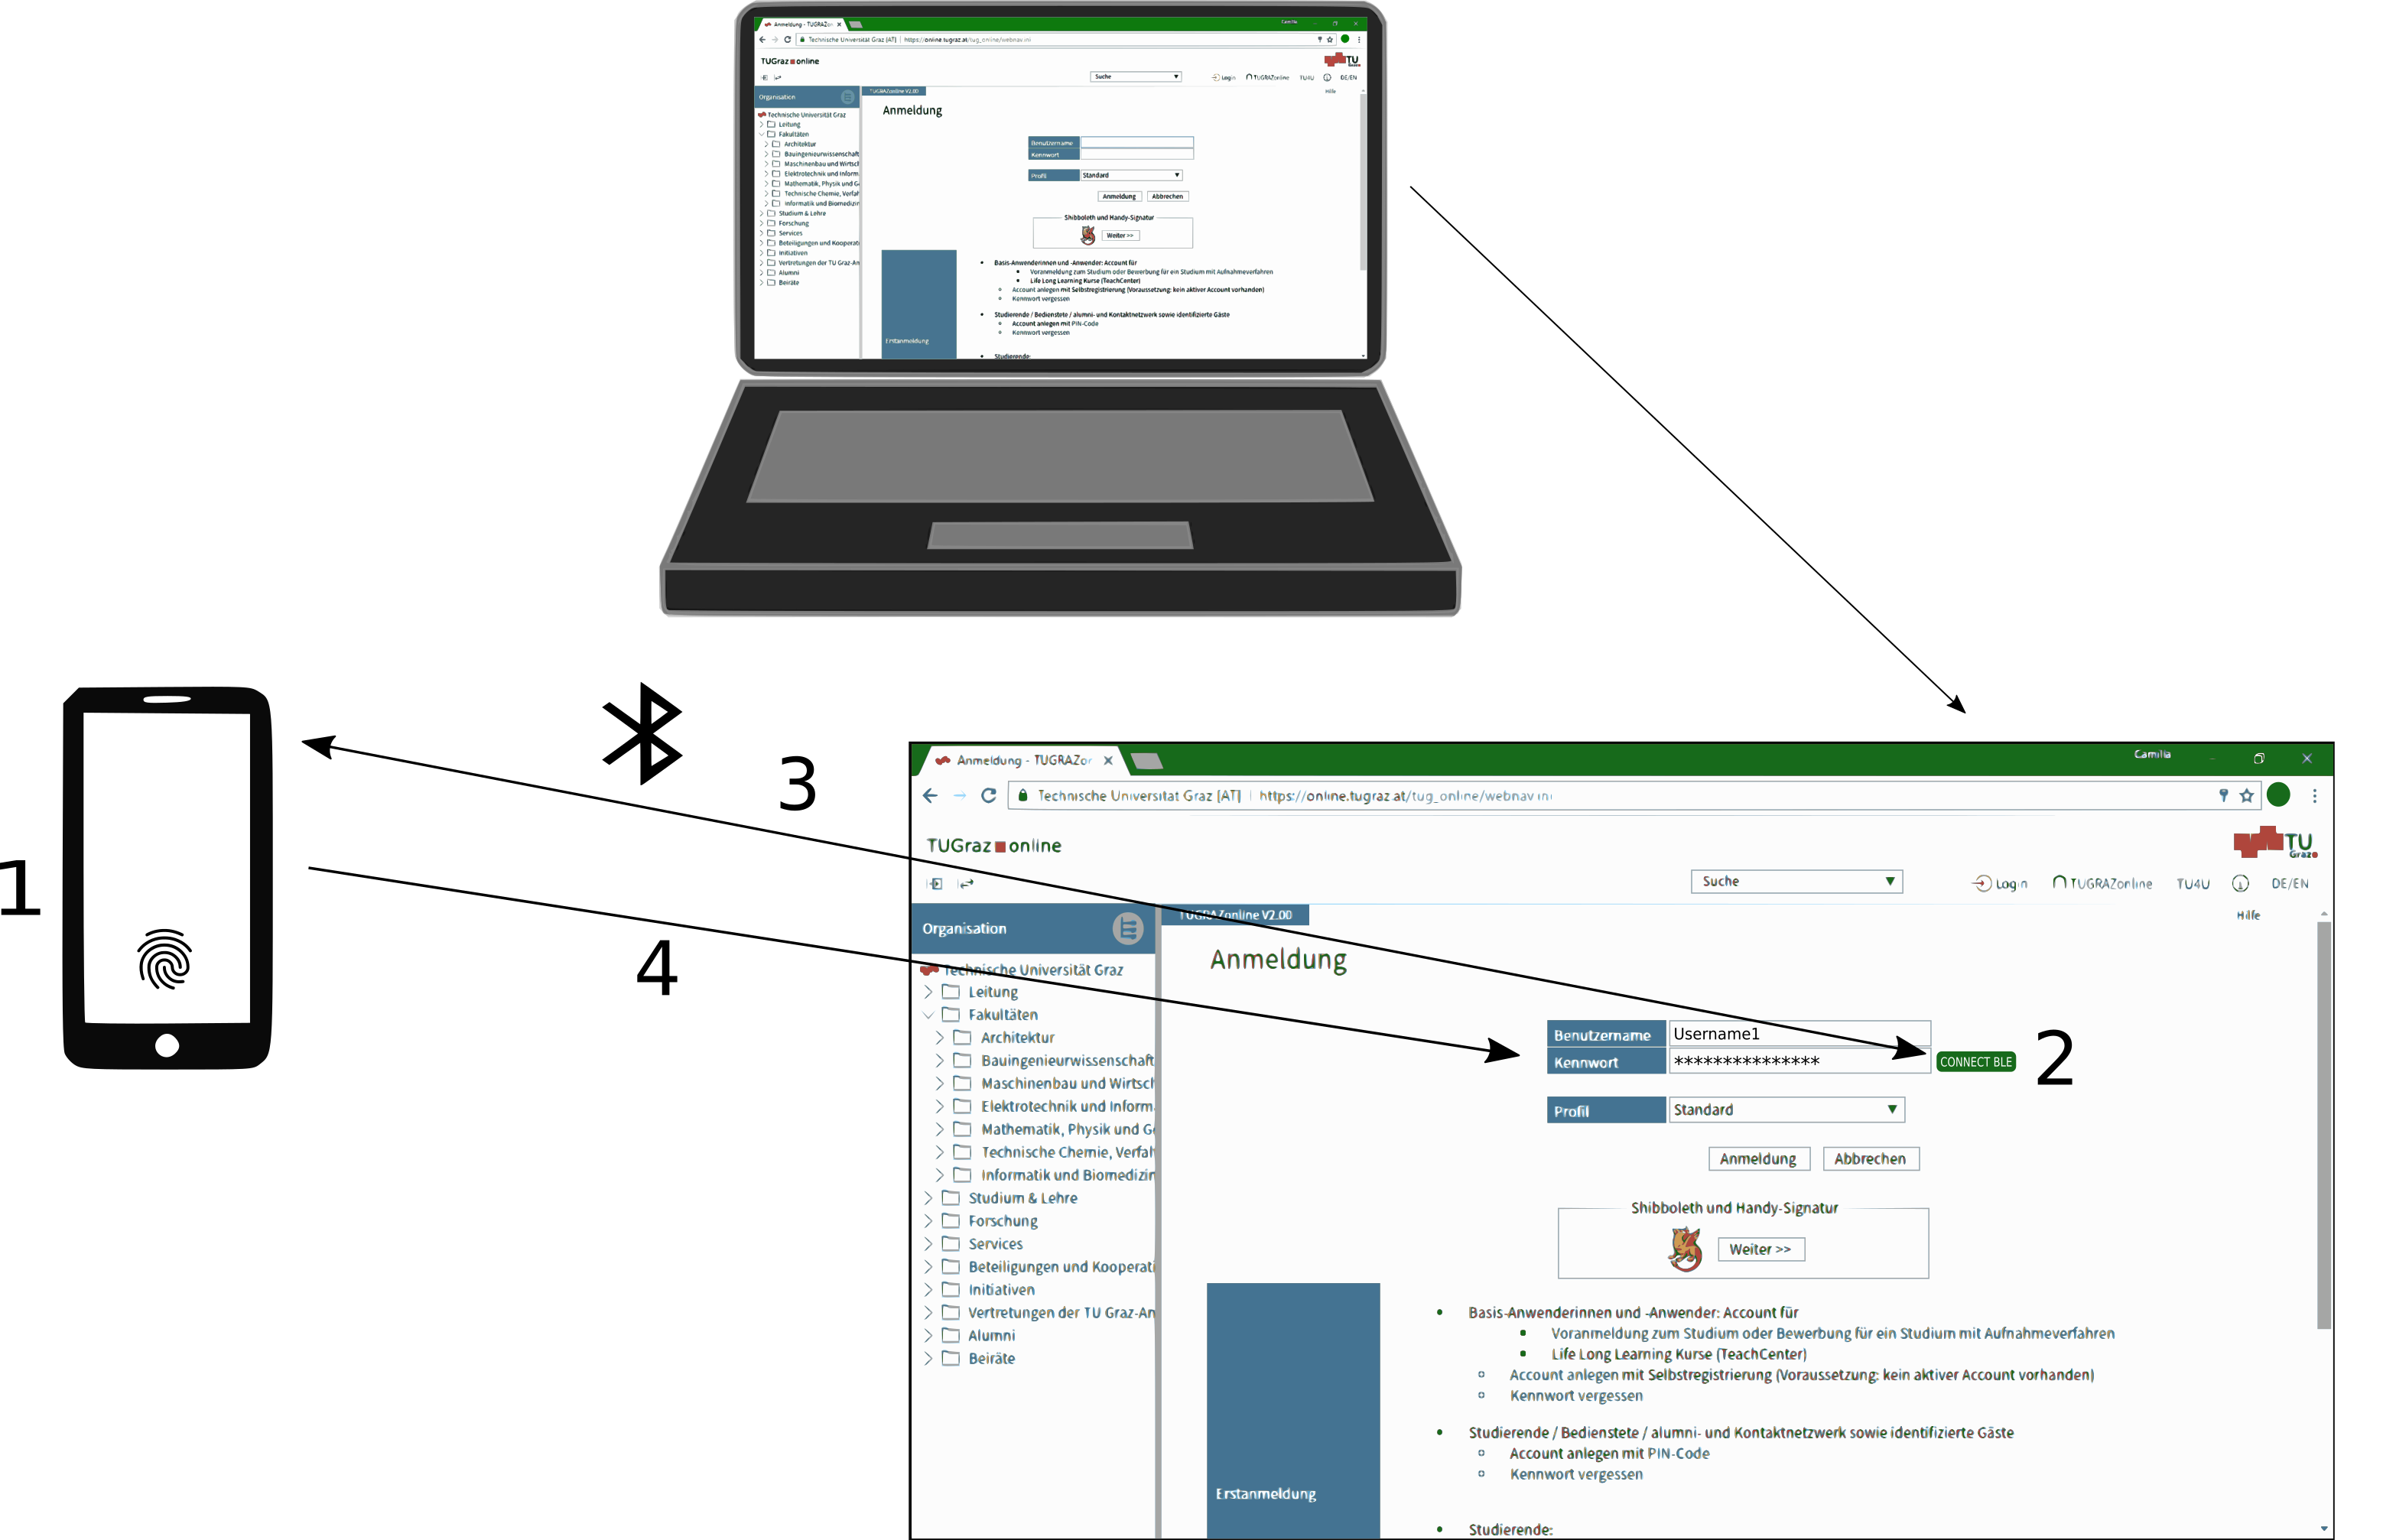
\includegraphics[width=14cm]{images/Communication.png}
    \caption[Workflow between Devices]{The workflow between the mobile device and the web browser.}
    \label{fig:comm}
\end{figure}
\vspace{0.3cm}



\noindent We implemented the application for \gls{api} level 23 and up using Android Studio as the IDE. One of the reasons for this decision is that Android supports native fingerprint reader support from that \gls{api} level, as stated in \cite{AndroidM}. The app consists of a main activity, which is seen in Figure \ref{fig:mainactivity}. It contains three different menu items: \textit{Accounts}, which provides the user with an interface to manage their login accounts, \textit{Connection}, where users can establish the Bluetooth connection to send login data to the web browser, and \textit{About}. We will go more into detail about the functionality of the activities \textit{Accounts} and \textit{Connection} in the following Sections. Subsequently, we will examine how the application handles data storage, encryption, and authentication in greater detail.

\begin{figure}[!htb]
\centering
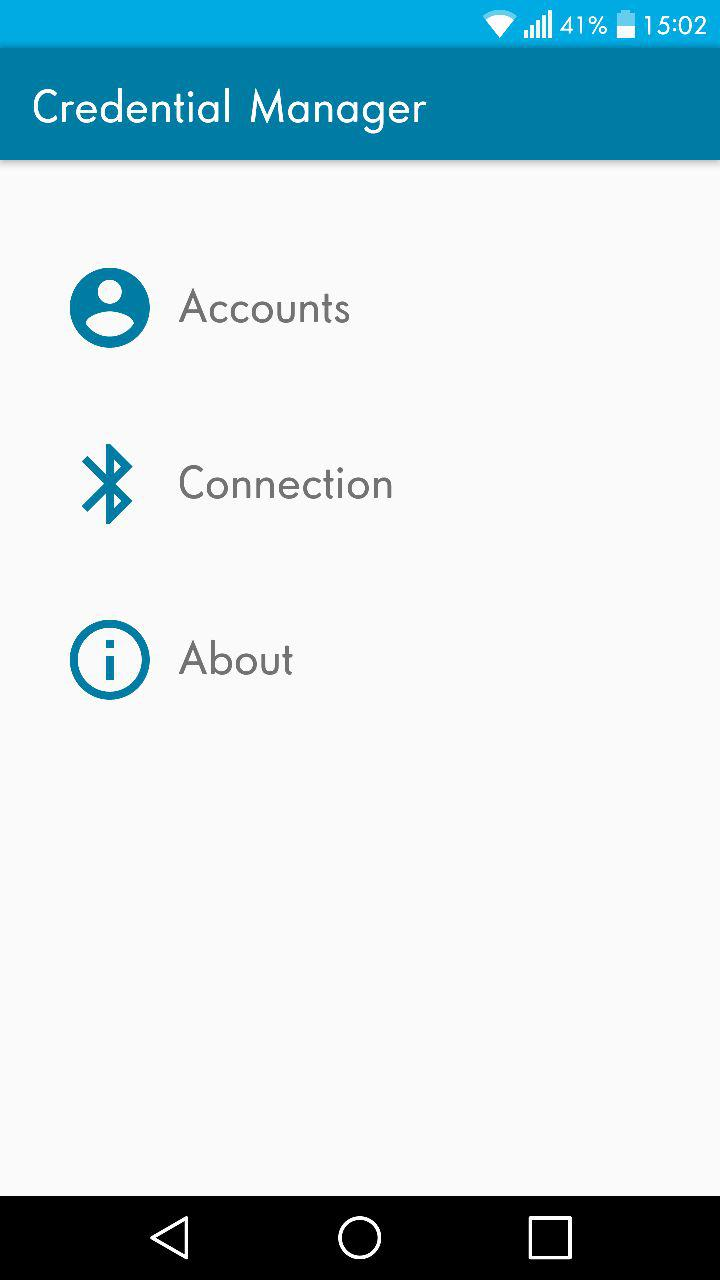
\includegraphics[width=4cm]{images/MainActivityNew}
\caption[Main Activity]{Main activity, which is shown at start up of the app}
\label{fig:mainactivity}
\end{figure}

%-------------------------------------------------------------------------------------

\subsection{Activity for managing Accounts}
By clicking on the menu item \textit{Accounts}, the user is asked to authenticate (cf. Section \ref{arch_authenticate}). Upon successful verification, the interface in Figure \ref{fig:accountactivity}\protect\subref{show_acc} is shown. It gives an overview of saved credentials. By clicking the button on the bottom right corner, the activity is switched to the activity shown in Figure \ref{fig:accountactivity}\protect\subref{add_acc}. Here the user can add a new accounts. Clicking the \texttt{save}-button encrypts and adds the credential to the database (cf. Section \ref{arch_encryption}).

When clicked on one of the existing credentials in the list, it takes the user to the interface shown in Figure \ref{fig:accountactivity}\protect\subref{change_acc}.  Here data can be changed and saved again. Also, the account can be deleted from the database. When deleting a credential, the user is asked to confirm their action via a prompt, as seen in Figure \ref{fig:accountactivity}\protect\subref{prompt_delete}.

\begin{figure}[!htb]
\centering
\subfloat[]{{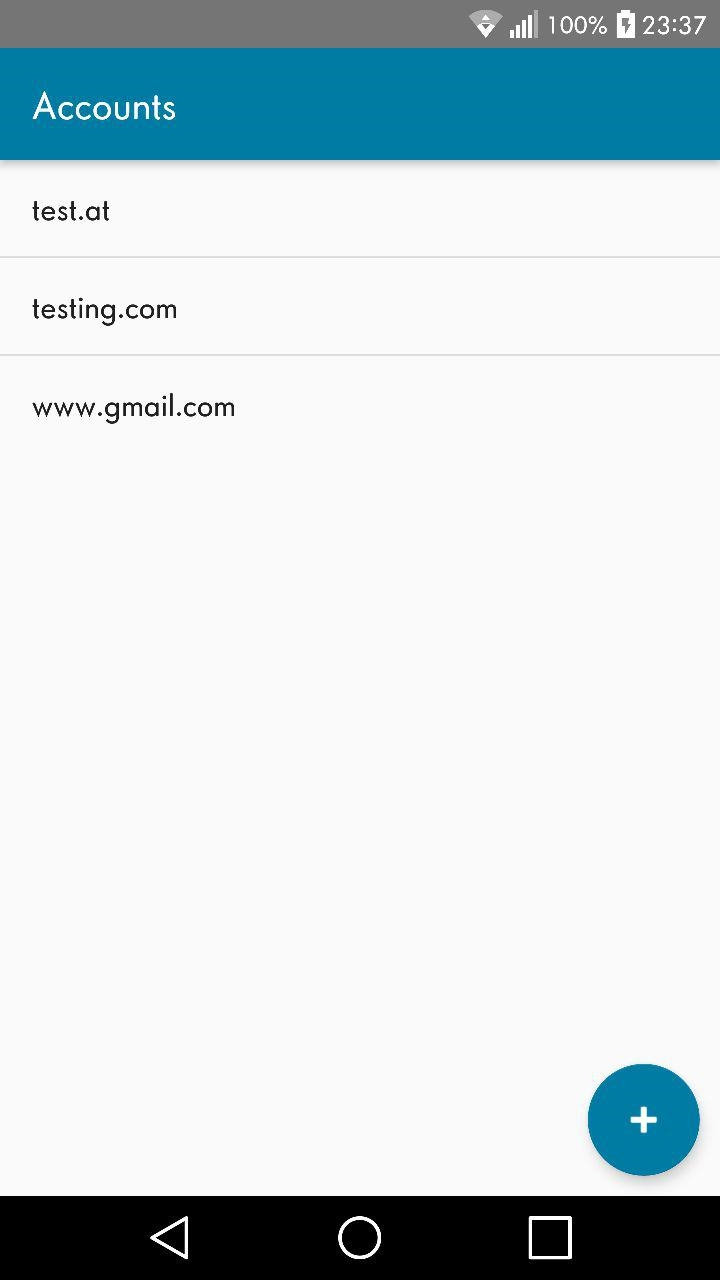
\includegraphics[width=3.5cm]{images/ShowAccountsActivity}\label{show_acc} }}
\qquad
\subfloat[]{{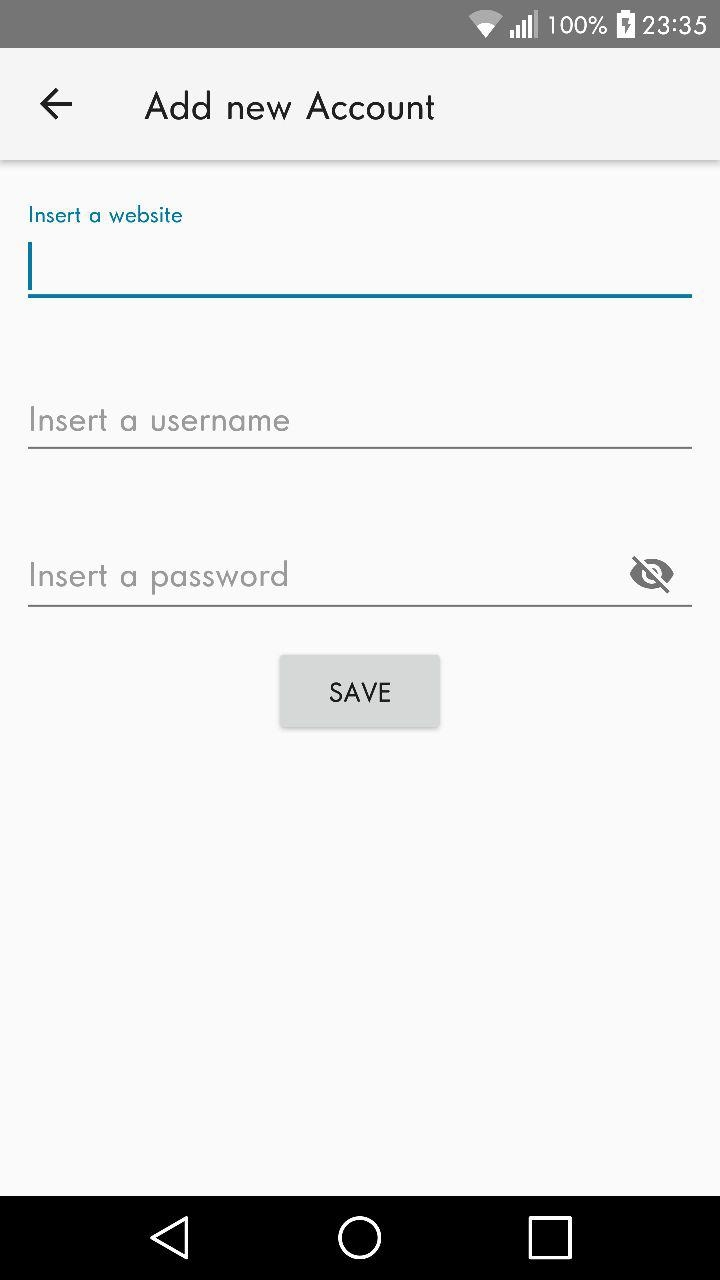
\includegraphics[width=3.5cm]{images/AddAccountActivity}\label{add_acc} }}
\qquad
\subfloat[]{{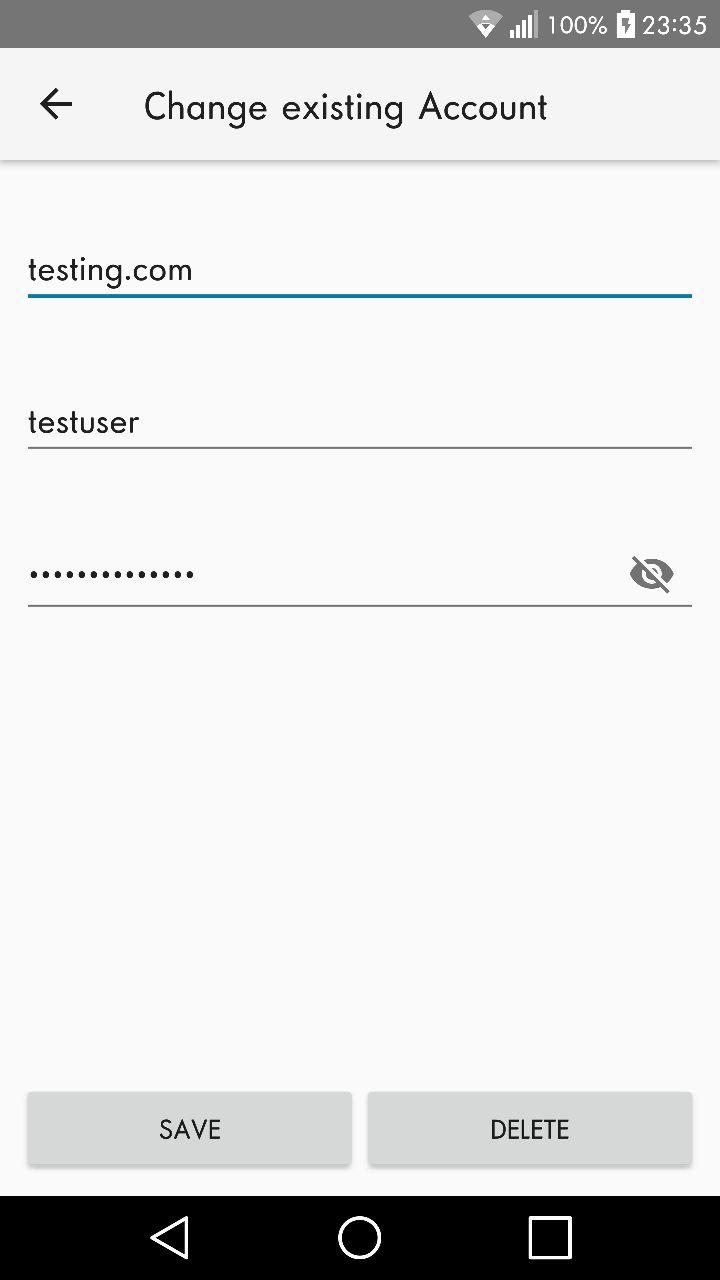
\includegraphics[width=3.5cm]{images/ChangeAccountActivity}\label{change_acc} }}
\qquad
\subfloat[]{{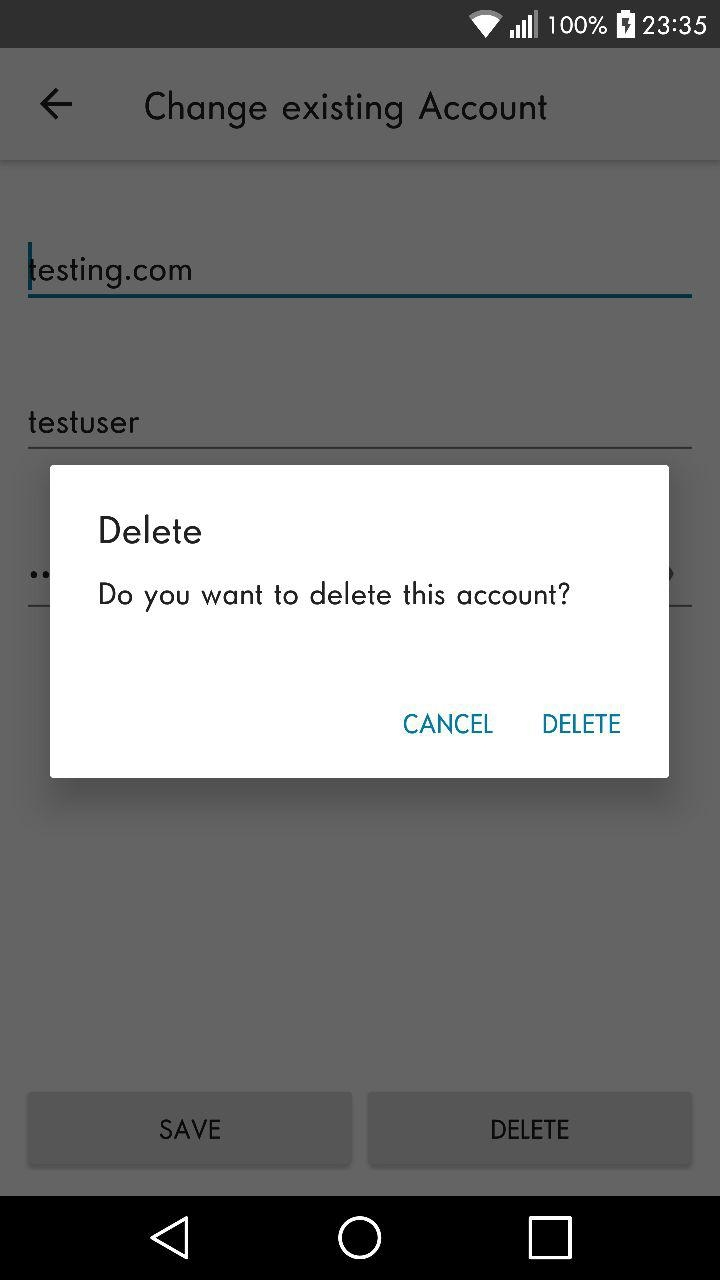
\includegraphics[width=3.5cm]{images/DeleteAccount}\label{prompt_delete} }}
\caption[Activity for managing Accounts]{Activity for managing Accounts; \protect\subref{show_acc}: listed accounts are shown. \protect\subref{add_acc}: interface where the user can add accounts. \protect\subref{change_acc}: the user can change a selected account. \protect\subref{prompt_delete}: user is asked to confirm before deleting the credential.}
\label{fig:accountactivity}
\end{figure}

%-------------------------------------------------------------------------------------

\subsection{Activity for Bluetooth Connection}
After selecting the menu item \textit{Connection}, the app checks immediately if Bluetooth is enabled. If it is not turned on, the user is asked via a prompt to enable Bluetooth as shown in Figure \ref{fig:connectionactivity}\protect\subref{prompt_bt}.
If the activation is denied, the application will return to the main activity with an error message, displayed in Figure \ref{fig:connectionactivity}\protect\subref{bt_notEnabled}. \\
Once Bluetooth is enabled, the accounts available for sharing are listed. At first, the application does not advertise any data. The user is asked to select an account to send to the Web Bluetooth \gls{api} as seen in Figure \ref{fig:connectionactivity}\protect\subref{not_advertising}. Before any credentials are shared, the user is asked to authenticate. This is done by scanning the fingerprint. Figure \ref{fig:connectionactivity}\protect\subref{advertising} shows that only after successful authentication the advertising starts.

\begin{figure}[!htb]
\centering
\subfloat[]{{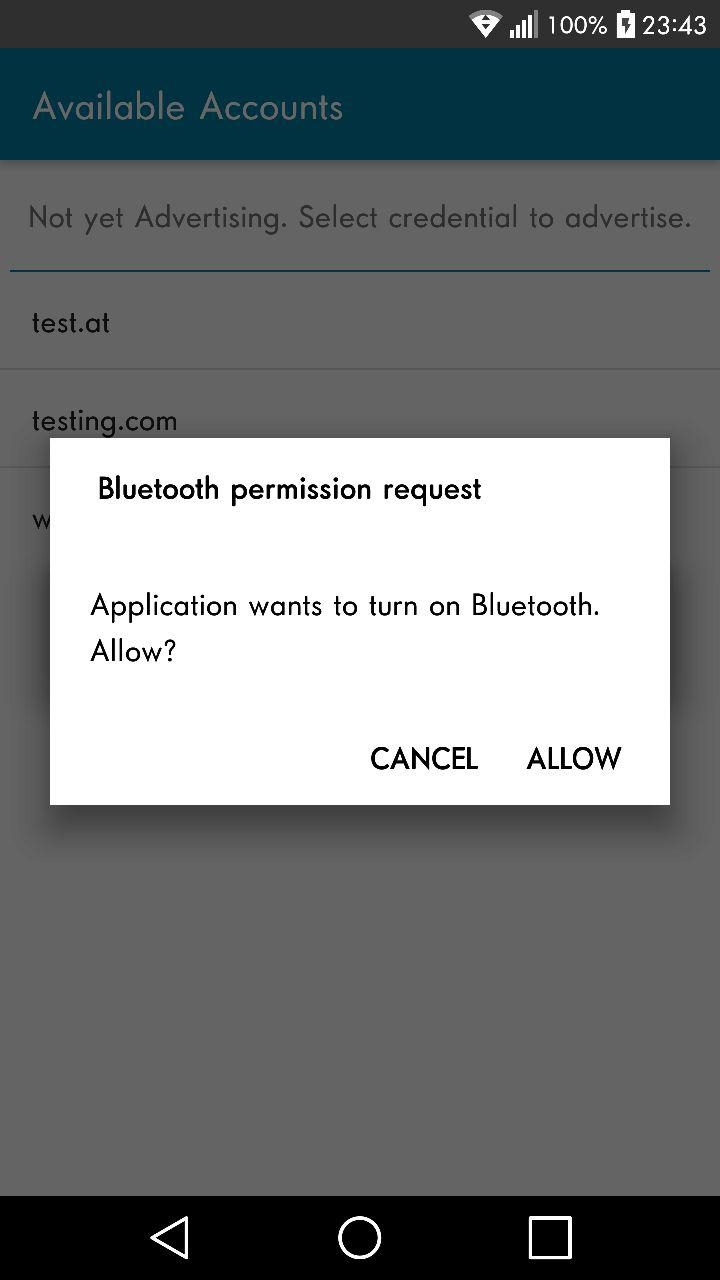
\includegraphics[width=3.5cm]{images/BT_english}\label{prompt_bt} }}
\qquad
\subfloat[]{{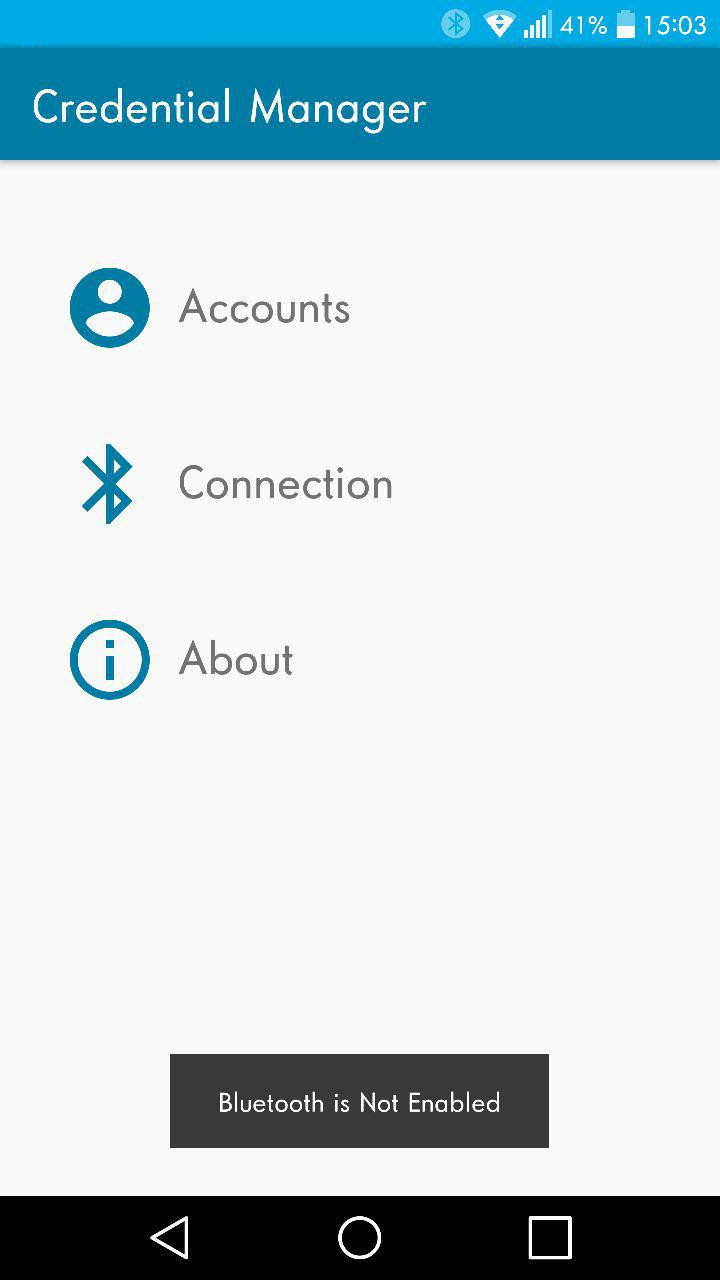
\includegraphics[width=3.5cm]{images/BTNotEnabledNew}\label{bt_notEnabled} }}
\qquad
\subfloat[]{{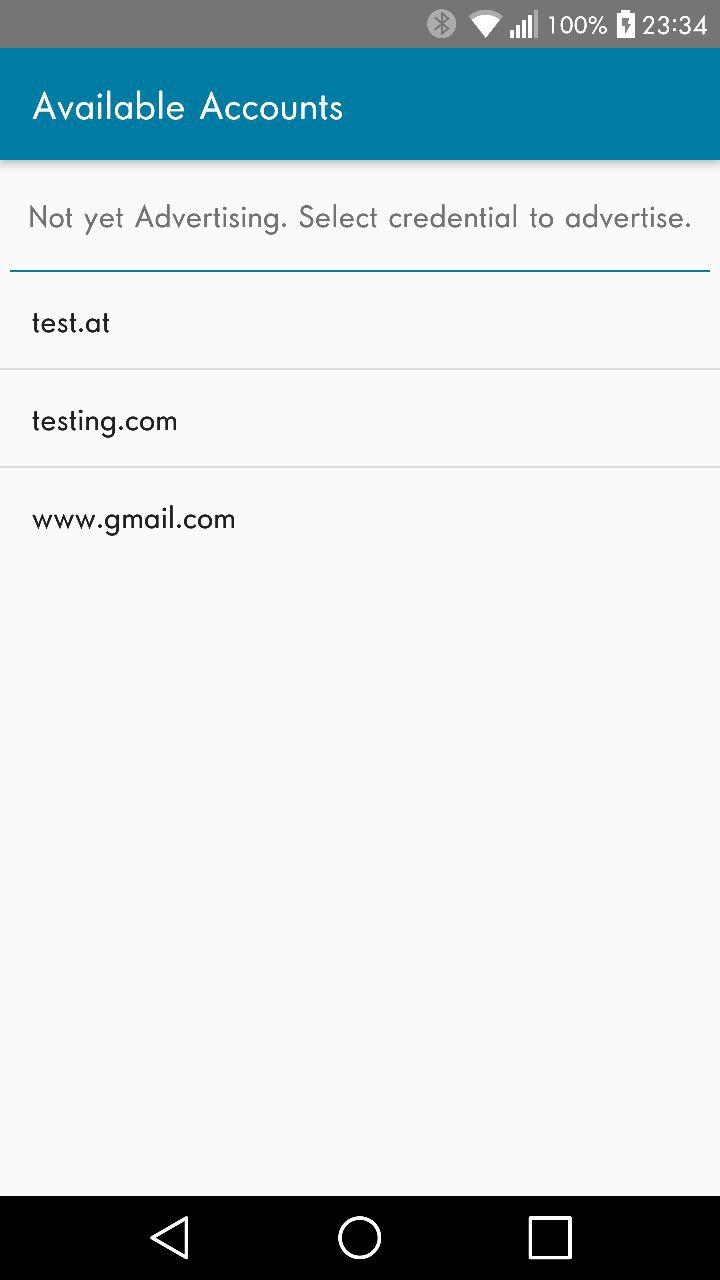
\includegraphics[width=3.5cm]{images/AvailableAccounts}\label{not_advertising} }}
\qquad
\subfloat[]{{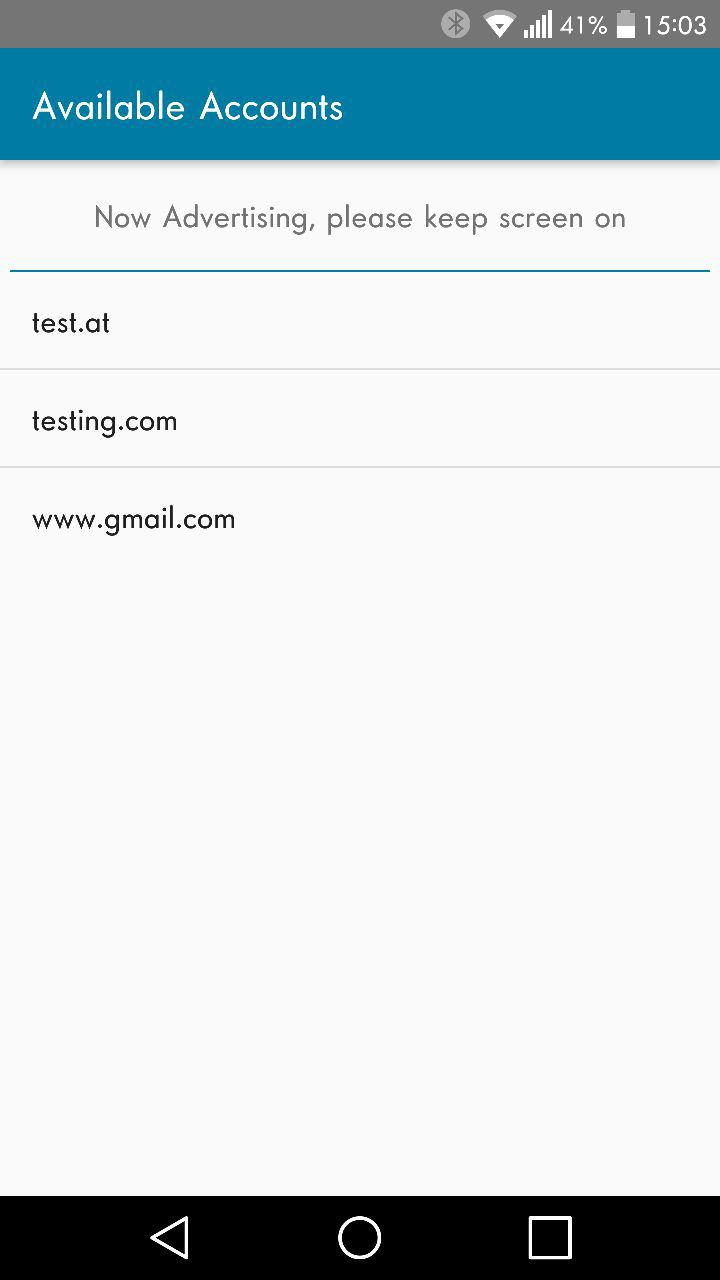
\includegraphics[width=3.5cm]{images/NowAdvertising}\label{advertising} }}
\caption[Activity for Bluetooth Connection]{Activity for Bluetooth Connection; \protect\subref{prompt_bt}: a prompt is shown to the user to enable Bluetooth. \protect\subref{not_advertising}: is shown when the application is not advertising. \protect\subref{advertising}: is shown after user selected a credential to send.}
\label{fig:connectionactivity}
\end{figure}

%-------------------------------------------------------------------------------------


\subsection{Storage using greenDao ORM}
Since one goal is to store user credentials on the phone, we need a suitable database structure. One option was a common SQLite database. SQLite databases use SQL queries to store, retrieve and delete data. However, SQL queries can be vulnerable to security attacks, for example, second-order SQL injections. As stated in \cite{Halfond2005}, a SQL injection is a type of attack where code is injected and the user's input is treated as part of the SQL code. A SQL injection exploits a security vulnerability in the database layer of an application. It is done by modifying input data which then alters the SQL query. This procedure increases the risk of storing data insecurely and may lead to a vulnerable application. \cite{katole2018detection} states that the risk of a SQL injection attack can increase due to not investing sufficient development time or lack of experience. We decided not to implement traditional SQL queries.

For this project, we use the \gls{orm} framework called greenDAO. It manages the tasks of storing, deleting, updating, and querying. The reason for choosing greenDAO is it has an overall good performance compared to different frameworks, according to \cite{Greendao}. \\
Before setting up the database, we included the greenDAO plugin. To set up the database, a DaoMaster had to be initialized. The DaoMaster is provided from the helper class \texttt{DevOpenHelper}, and handles the database set up and creates DaoSessions. Listing \ref{lst:db_master} shows this process.

\begin{lstlisting}[float,floatplacement=h, caption=Creation of Database, label=lst:db_master]
DaoMaster.DevOpenHelper helper = 
        new DaoMaster.DevOpenHelper(this,"credentials-db");
Database db = helper.getWritableDb();
daoSession = new DaoMaster(db).newSession();
\end{lstlisting}
%\vspace{0.5cm}

A DaoSession, on the other hand, manages the DAO object. It is an entity that we store in the database. DAO objects are created from a Java class. To define a Java class as a database-backed entity, annotations to the class-header and the class members must be added. The class members define the columns of the database. Afterward, the greenDAO generator automatically generates all the required methods. After this process is done, instances of the class can be stored in the greenDAO database \cite{Greendao}.

\subsubsection*{Load, insert and delete a database entry}
As mentioned before, the DaoSession manages DAO objects and they, in turn, handle all operations of the database. With the start of the application, the database is opened, and a new DaoSession is instantiated. To manage all interactions of DAO objects, we defined a database helper class. \\
Listing \ref{lst:db_insert} shows an example of how one credential is inserted in the database. The DaoSession calls the DAO object, and the object handles the insert method to store data in the database. The load and delete methods use the DaoSession as well. 

\begin{lstlisting}[float,floatplacement=h, caption= Insert Entry in Database, label=lst:db_insert]
public void insertNewAccount(Account account) {
    AccountDao accountDao = this.daoSession.getAccountDao();
    accountDao.insert(account);
}
\end{lstlisting}
\vspace{0.5cm}

The database created by the application lies in persistent memory of the mobile device, and can only be accessed from our app (cf. Section \ref{limitations}). In case of an attack even if the database content is dumped, the attacker is left with encrypted data. In Section \ref{arch_encryption} we discuss how data is encrypted before inserting in the database and decrypted again when fetching from it. \\

%-------------------------------------------------------------------------------------

\subsection{Encryption of Data}\label{arch_encryption}
For en- and decryption of sensitive data there exist different possibilities. One option of storing passwords is hashing and storing the hash in the database. SHA256 or SHA512 are some hash algorithms. However, by hashing data for encryption, data can be recovered by multiple different attacks such as Brute Force or Dictionary attack, as mentioned in \cite{ertaul2016implementation}. Hence, storing passwords with fast hash algorithms is not advisable. \\
Another way to store sensitive data is to hash it with a random string of bits, called \textit{salt}. The salt is stored with the hash of the plaintext. Still, this approach can also become vulnerable to Dictionary Attacks, as stated in \cite{3wrongways}. \\
Nowadays it is common to use a key derivation function to store passwords securely. They must generate a strong key that is secure against various attacks. Latest key derivation functions are \gls{pbkdf2}, Bcrypt, and Scrypt. As mentioned in \cite{ertaul2016implementation}, their security is strong.
However, \gls{pbkdf2} requires the user's input to generate the encryption key. Hence, it depends on the password chosen by the user, as stated in \cite{Agilebits}. Furthermore, \cite{YanBAG04} shows that users create passwords that may not be secure. In case of an easy to guess password, \gls{pbkdf2} can become target of brute force attacks with GPUs as shown in \cite{DurmuthGKPYZ12}.

Our goal is to provide secure en- and decryption without depending on the user's input. Also, all encryption tasks take place on the mobile phone, and there is no need for distribution of a public key component. Hence, the same key can be used for encryption and decryption. As discussed in \cite{bala2015asymmetric}, symmetric key algorithms are efficient and secure and provide fast execution of computation. Also, they consume fewer resources such as memory and processor time. \\ Therefore, we decided to encrypt data using the AES algorithm and \gls{gcm} as our cipher mode. \gls{gcm} provides confidentiality, integrity, and authenticity, as stated in \cite{AESJavaAndroid}.

\gls{gcm} uses the Counter Mode (CTR) internally. A counter value for each block is encrypted and only uses as many bits as required from the last block. \cite{AESJavaAndroid} states that this process turns the block cipher into a stream cipher, and no padding is required. \\
\cite{fedler2013padding} discusses thoroughly that CBC mode is prone to padding attacks. The CBC mode works with fixed size input blocks, and because input data can vary in size, padding is required. \\
Hence, we decided to use \gls{gcm} as our cipher mode. \gls{gcm} takes as input an \gls{iv}, a plaintext, and \gls{aad}. As discussed in \cite{mcgrew2004galois}, the \gls{aad} is not encrypted and can have a length of $0$ up to $2^{64}$ bits. \\
We instantiated the cipher, as seen in Listing \ref{lst:cipher}.

\begin{lstlisting} [float,floatplacement=!htb, caption=Instantiation of Cipher, label=lst:cipher]
final Cipher cipher = Cipher.getInstance("AES/GCM/NoPadding");
\end{lstlisting}

In this project, we passed the plaintext and the \gls{iv}. According to \cite{dworkin2007sp}, the output of encryption is the ciphertext and an authentication tag. The authentication tag contains information, that is associated with the encrypted data. \cite{AESJavaAndroid} states, the authentication tag helps to identify an unauthorized change. As discussed in \cite{dworkin2007sp}, when decrypting data, \gls{gcm} expects the \gls{iv}, a ciphertext, the authentication tag, and the AAD, if it has been passed during encryption. Only if the authentication tag calculated during encryption and the one passed are identical, the plaintext is returned.

Important for the Android implementation of \gls{gcm} is the length of the \gls{iv}. National Institute of Standards and Technology \cite{dworkin2007sp} recommends 96 bits for the \gls{iv} to be fast and secure. To ensure that a unique \gls{iv} is used with every encryption, a new one is generated upon each call of the encrypt method. Afterward, we concatenate the \gls{iv} with the ciphertext. Before decryption, the \gls{iv} is separated from the ciphertext again. We created the \gls{iv} using the strong random number generator \textit{SecureRandom} from the Android Library \cite{SecureRandom}.

Android insists on using their default method \texttt{cipher.getIV();} for generating the \gls{iv}. However, as mentioned in \cite{DefaultIV}, using the default \gls{iv} may not be secure due to old versions of Android returning an all $0$ \gls{iv}, which leads to the same key. Reusing an \gls{iv} results in a vulnerable implementation and compromises the security of data. \cite{dworkin2007sp} states that the \gls{iv} being unique is almost as important as the key being secret. \\
To ensure random \glspl{iv}, we decided to provide the \gls{iv} by SecureRandom. 

The Android OS throws an exception if not using the provided method \texttt{cipher.getIV()}. To solve this problem, we set the \textit{setRandomizedEncryptionRequired()} property to \textit{false} when we generated the key, which is shown in Listing \ref{lst:key}. This way Android allows using our generated \gls{iv} as shown in \cite{SecretsInAndroid}. \\
After generation of the key and successful encryption, it is crucial to store the key securely. We rely on the Android Keystore for this task. Chapter \ref{arch_keystore} discusses storage of the key. \\


\begin{lstlisting} [float,floatplacement=!htb, caption=Setting Properties of Secret Key, label=lst:key]
SpecBuilder.setKeySize(128)
    .setBlockModes(KeyProperties.BLOCK_MODE_GCM)
    .setEncryptionPaddings(KeyProperties.ENCRYPTION_PADDING_NONE)
    .setRandomizedEncryptionRequired(false);
\end{lstlisting}



%-------------------------------------------------------------------------------------

\subsection{Secure Storage of Secret Key} \label{arch_keystore}
As stated in \cite{dworkin2007sp} and \cite{CooijmansRP14},  in practice the secrecy of the key and secure storage are crucial. If the key can be retrieved from the device, all ciphertexts can be decrypted easily. Therefore, we need a system to ensure secure storage of the key.

The \textit{AndroidKeystore} system allows secure storage of cryptographic keys. As mentioned in \cite{HWBKeyStore}, applications use this Android Framework \gls{api} to access Keystore functionality. According to \cite{AndroidKeyStoreSystem}, the AndroidKeystore lets an application store and manage its credentials while making sure no other application can access them.

To store the cryptographic key in a secure manner, we used the hardware-based security feature provided by a specific realization of the AndroidKeystore. The availability of the hardware-based security feature depends on the device manufacturer. 
On devices equipped with a Qualcomm processor with TrustZone Technology, the AndroidKeystore is automatically stored in the \acrfull{tee}. As described in \cite{CooijmansRP14}, modern mobile phones' processors are equipped with ARM TrustZone Technology that separates the hardware into two \glspl{os}: a secure world \gls{os} and normal \gls{os}. The secure world \gls{os} is also known as a \gls{tee}. The \gls{tee} ensures that data cannot be extracted from this trusted environment. Hence, keys stored in the \gls{tee} are challenging to be retrieved.
As of this writing, \cite{SecureDataEncryption} claims that it represents the most secure option to store keys. If a \gls{tee} is not supported, the keys are stored in a system provided emulated software environment. However, keys will be removed when deleting the application that created them.

Before we can generate a key or use it for encryption, we must instantiate and load the Keystore. According to \cite{CooijmansRP14}, a key is stored into the Keystore under a given identifier, also known as \textit{alias}. The alias is a string that defines a reference to the key. All cryptographic operations are done in the background, and key material is never exposed. Hence, the alias is needed everytime data is en- and decrypted. \\
Also, the lock screen must be set in order to reference the key. The KeyguardManager is used for this process. The method \texttt{isDeviceSecure()} returns if the device is secured with a PIN, pattern or password. If the device is not locked, the AndroidKeystore is not instantiated, and cryptographic calculations cannot take place. \\



%-------------------------------------------------------------------------------------

\subsection{Authentication through Biometrics} \label{arch_authenticate}
To securely protect user credentials, the app uses biometric authentication. As biometric authentication, we use the user's fingerprint. Whenever the user wants to access or send credentials, the application requires fingerprint authentication from the user.

For this process, an instance of the Android class \textit{FingerprintManager} is required. As described in \cite{FingerprintManager}, the class handles accesses to the fingerprint hardware. Before the actual authentication can take place, the application checks the following requirements. \\
Firstly, the application checks if a fingerprint sensor is available. The method \texttt{isHardwareDetected()} is called on the FingerprintManager to ensure the device supports fingerprint scanning. \\
The next requirement is the permission to use fingerprint scanning. This must be granted by the Android permission system, which is discussed in Section \ref{limitations}. \\
Also, the user must have at least one fingerprint registered on the device, as stated in \cite{FingerprintTutorial}. To ensure that fingerprints are registered, the FingerprintManager uses the method \texttt{hasEnrolledFingerprints()}. If no fingerprints are saved, a message is displayed as shown in Figure \ref{fig:authentication}\protect\subref{auth_none}. \\
Before starting authentication via fingerprint, the application makes sure the lock screen is secured. This is done with the Android class \texttt{KeyguardManager} \cite{KeyguardManager}. The KeyguardManager provides access to the lock screen and checks if a PIN, password or pattern is set or if the SIM card is locked. The mobile device must be secured for the authentication process to proceed.

As mentioned above, upon every request to retrieve credentials the user has to re-authenticate. This security mechanism can protect from an unintentional distribution of sensitive data. Therefore, the risk of threatened security can be reduced whenever the user left their phone unattended with the open application. \\

\begin{figure}[!htb]
\centering
\subfloat[]{{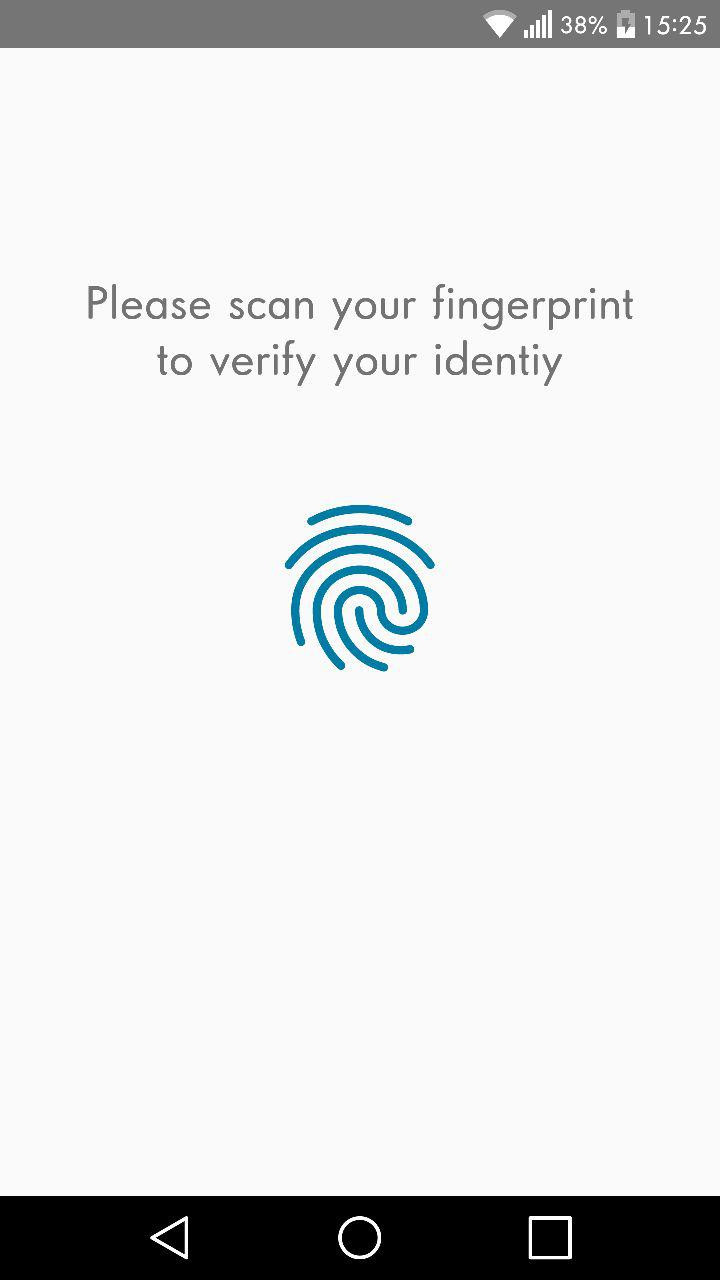
\includegraphics[width=3.5cm]{images/AuthenticationScreenNew}\label{auth_screen} }}
\qquad
\subfloat[]{{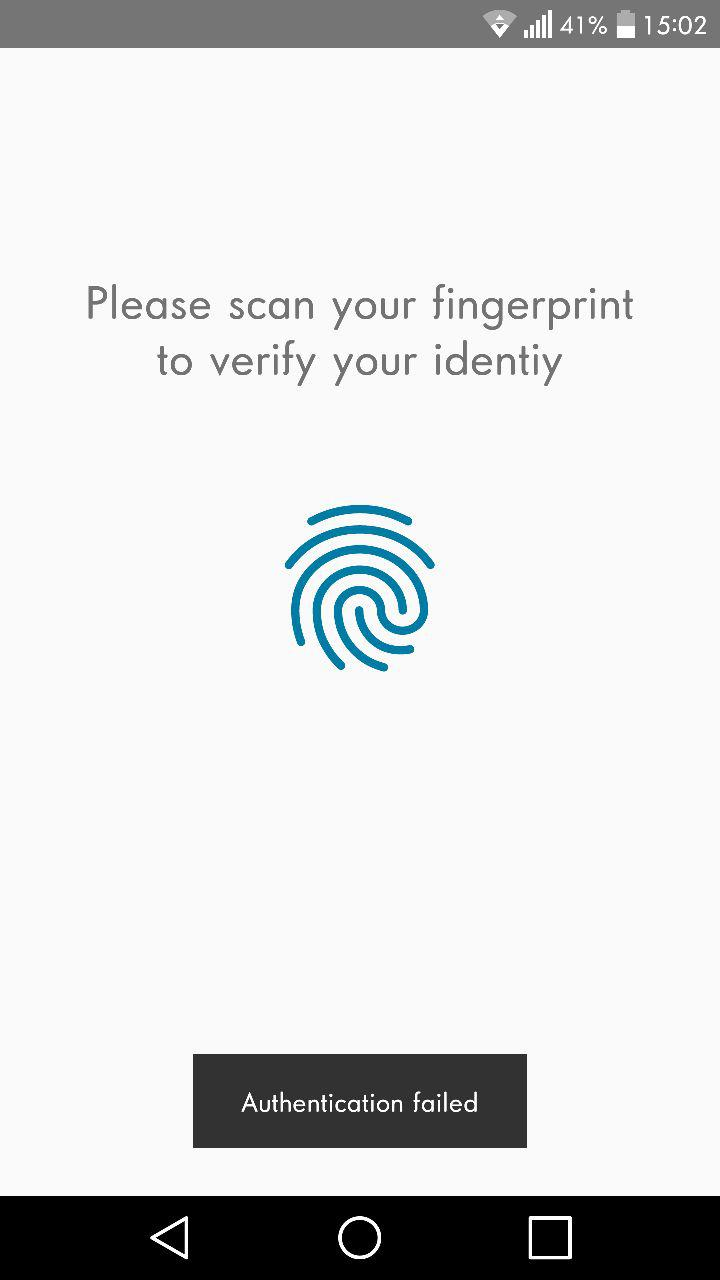
\includegraphics[width=3.5cm]{images/AuthenticationFailedNew}\label{auth_fail} }}
\qquad
\subfloat[]{{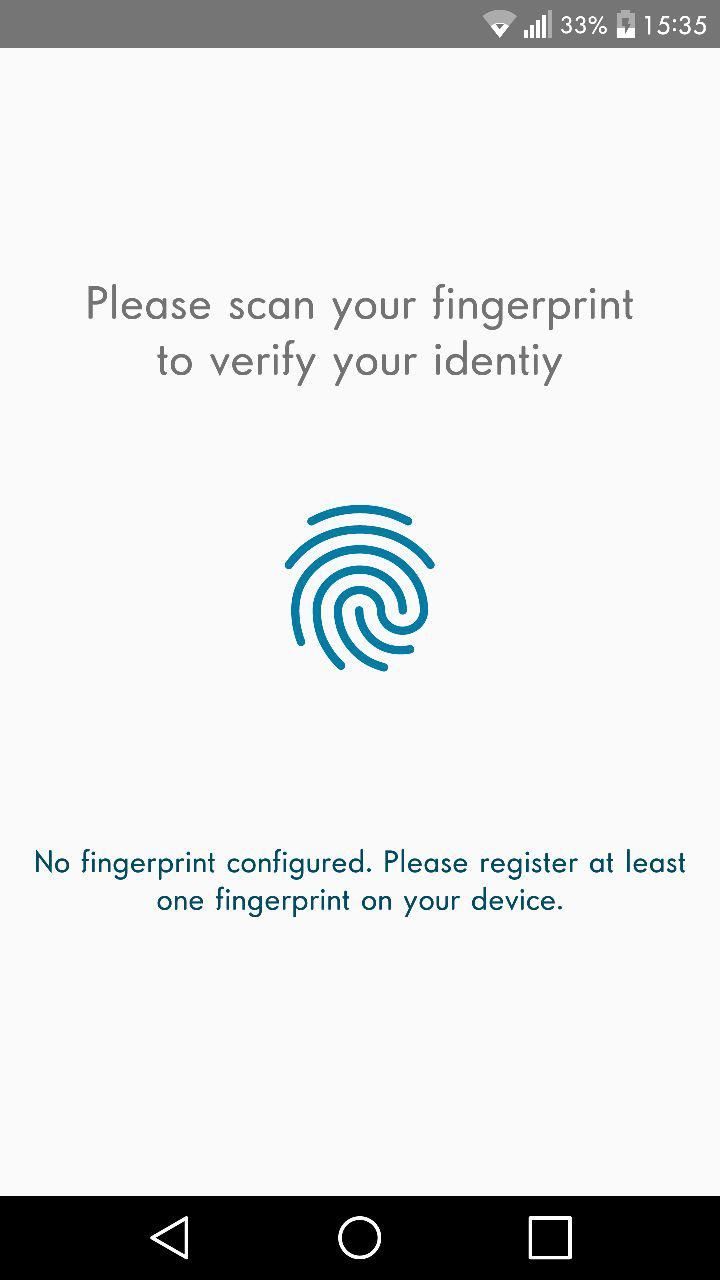
\includegraphics[width=3.5cm]{images/NoFingerprintRegistered}\label{auth_none} }}
\caption[Activity for Authentication]{Activity for Authentication; \protect\subref{auth_screen}: the user is asked to auhenticate. \protect\subref{auth_fail}: authentication failes if incorrect fingerprint is scanned. \protect\subref{auth_none}: is shown if no fingerprints are registered on the device.}
\label{fig:authentication}
\end{figure}

%-------------------------------------------------------------------------------------

\subsection{Chrome Extension with the Web Bluetooth API}
After discussing in depth the credential storage, encryption, and authentication, we will describe the communication of the extension and the Android application.

In addition to the application, we implemented an extension for the Chrome browser. Chrome exposes a dedicated Web Bluetooth \gls{api} to support a \gls{ble} connection \cite{WebBTAPI}. This allows websites to communicate with a near \gls{ble} device. Typically a \gls{ble} device advertises characteristics, while the Web Bluetooth \gls{api} consumes them.

The workflow is as follows: first, the application advertises a specific service containing the credentials. Services are specified by a \gls{uuid} and can advertise characteristics and descriptors. To distinguish our custom service from other \gls{ble} services we defined a \gls{uuid} in the code. The extension will only connect to the service that matches the defined \gls{uuid}. Once found, the connection of the Bluetooth devices takes place. Only after the devices have been paired, the Web Bluetooth \gls{api} can read the characteristics. Each characteristic has an own \gls{uuid}. This helps to distinguish them easily. We defined the username and password as our characteristics. They are retrieved from the service with the method \texttt{service.getCharacteristic();}. According to \cite{WebBTAPI}, to read the values, the Web Bluetooth \gls{api} uses the method \texttt{characteristic.readValue();} .
